\chapter{L2L2} \label{chap:L2L2}

\begin{figure}[!ht] 
    \centering
    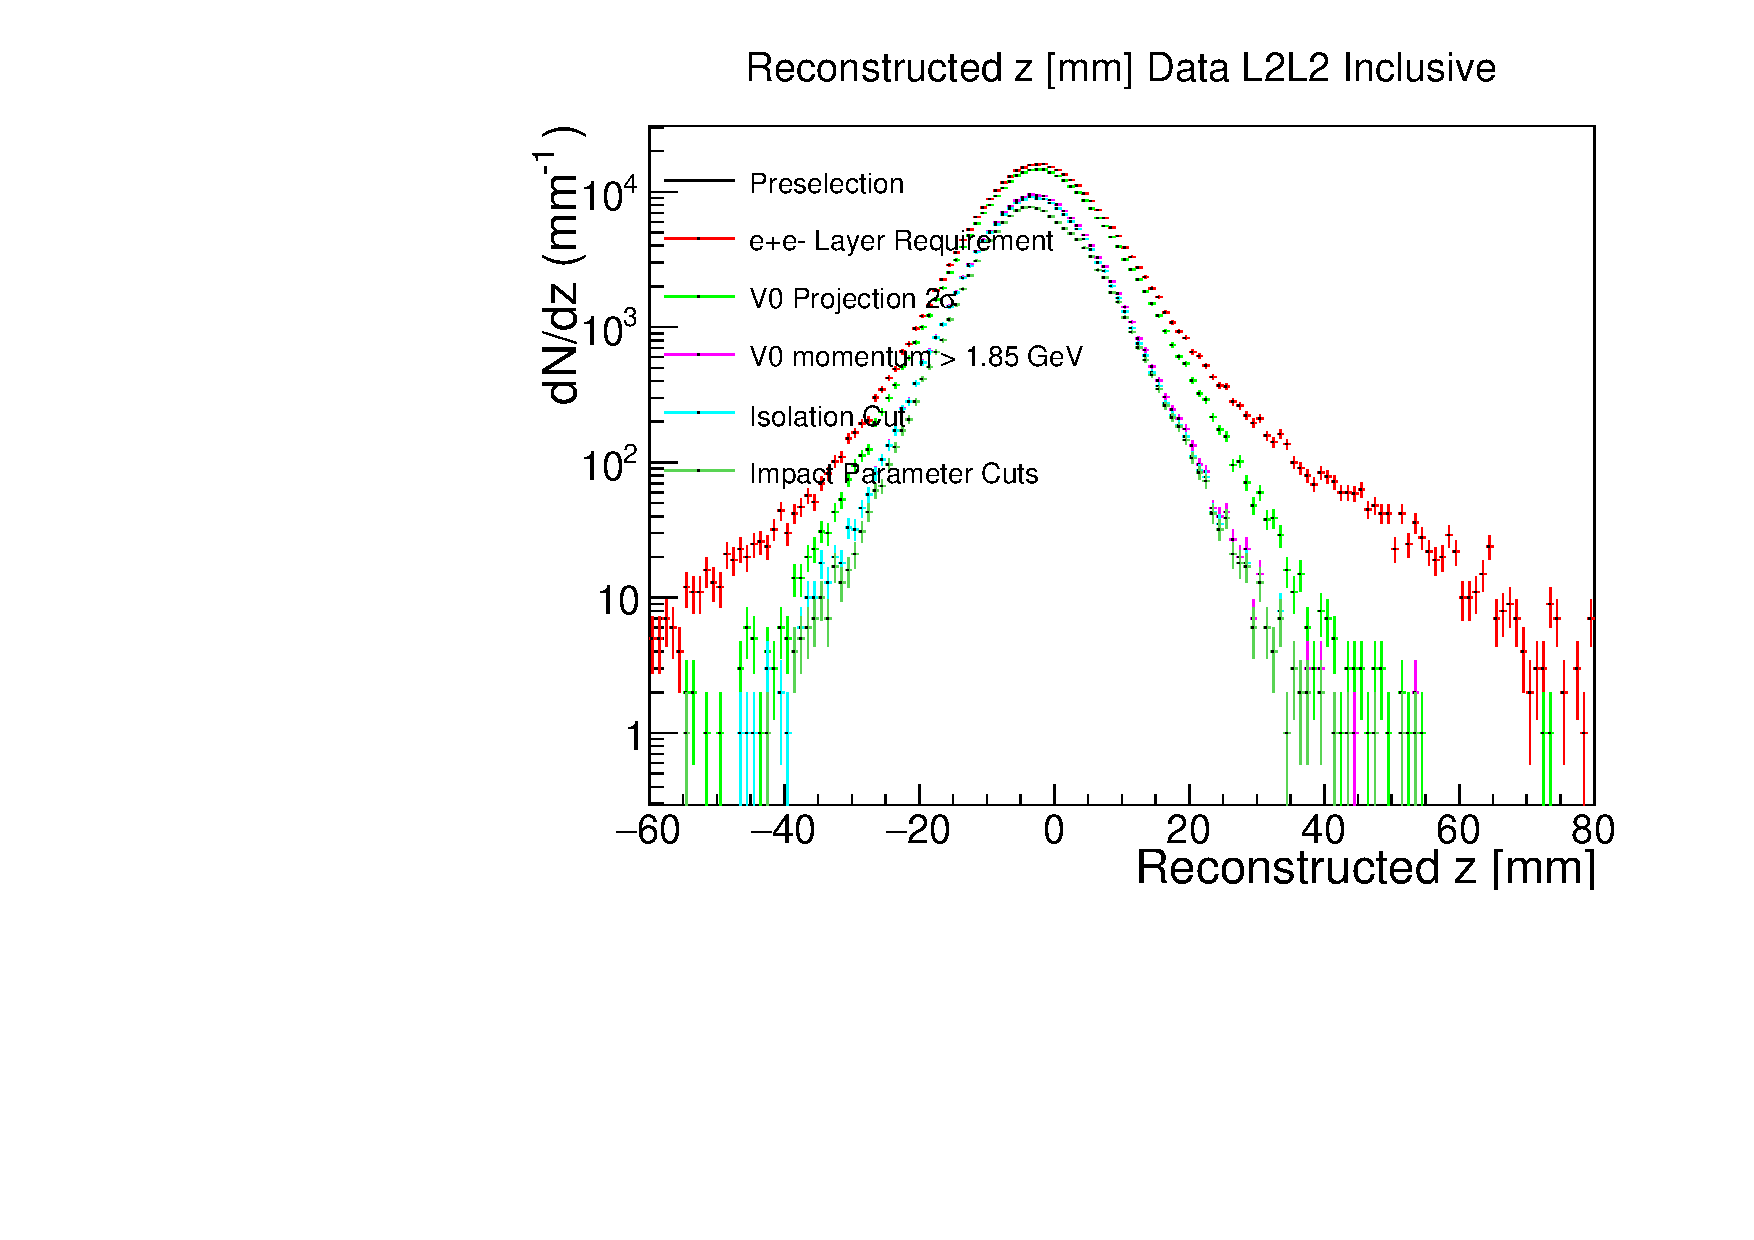
\includegraphics[width=.45\textwidth]{figs/selection/10per_L2L2_cutflow.pdf}
    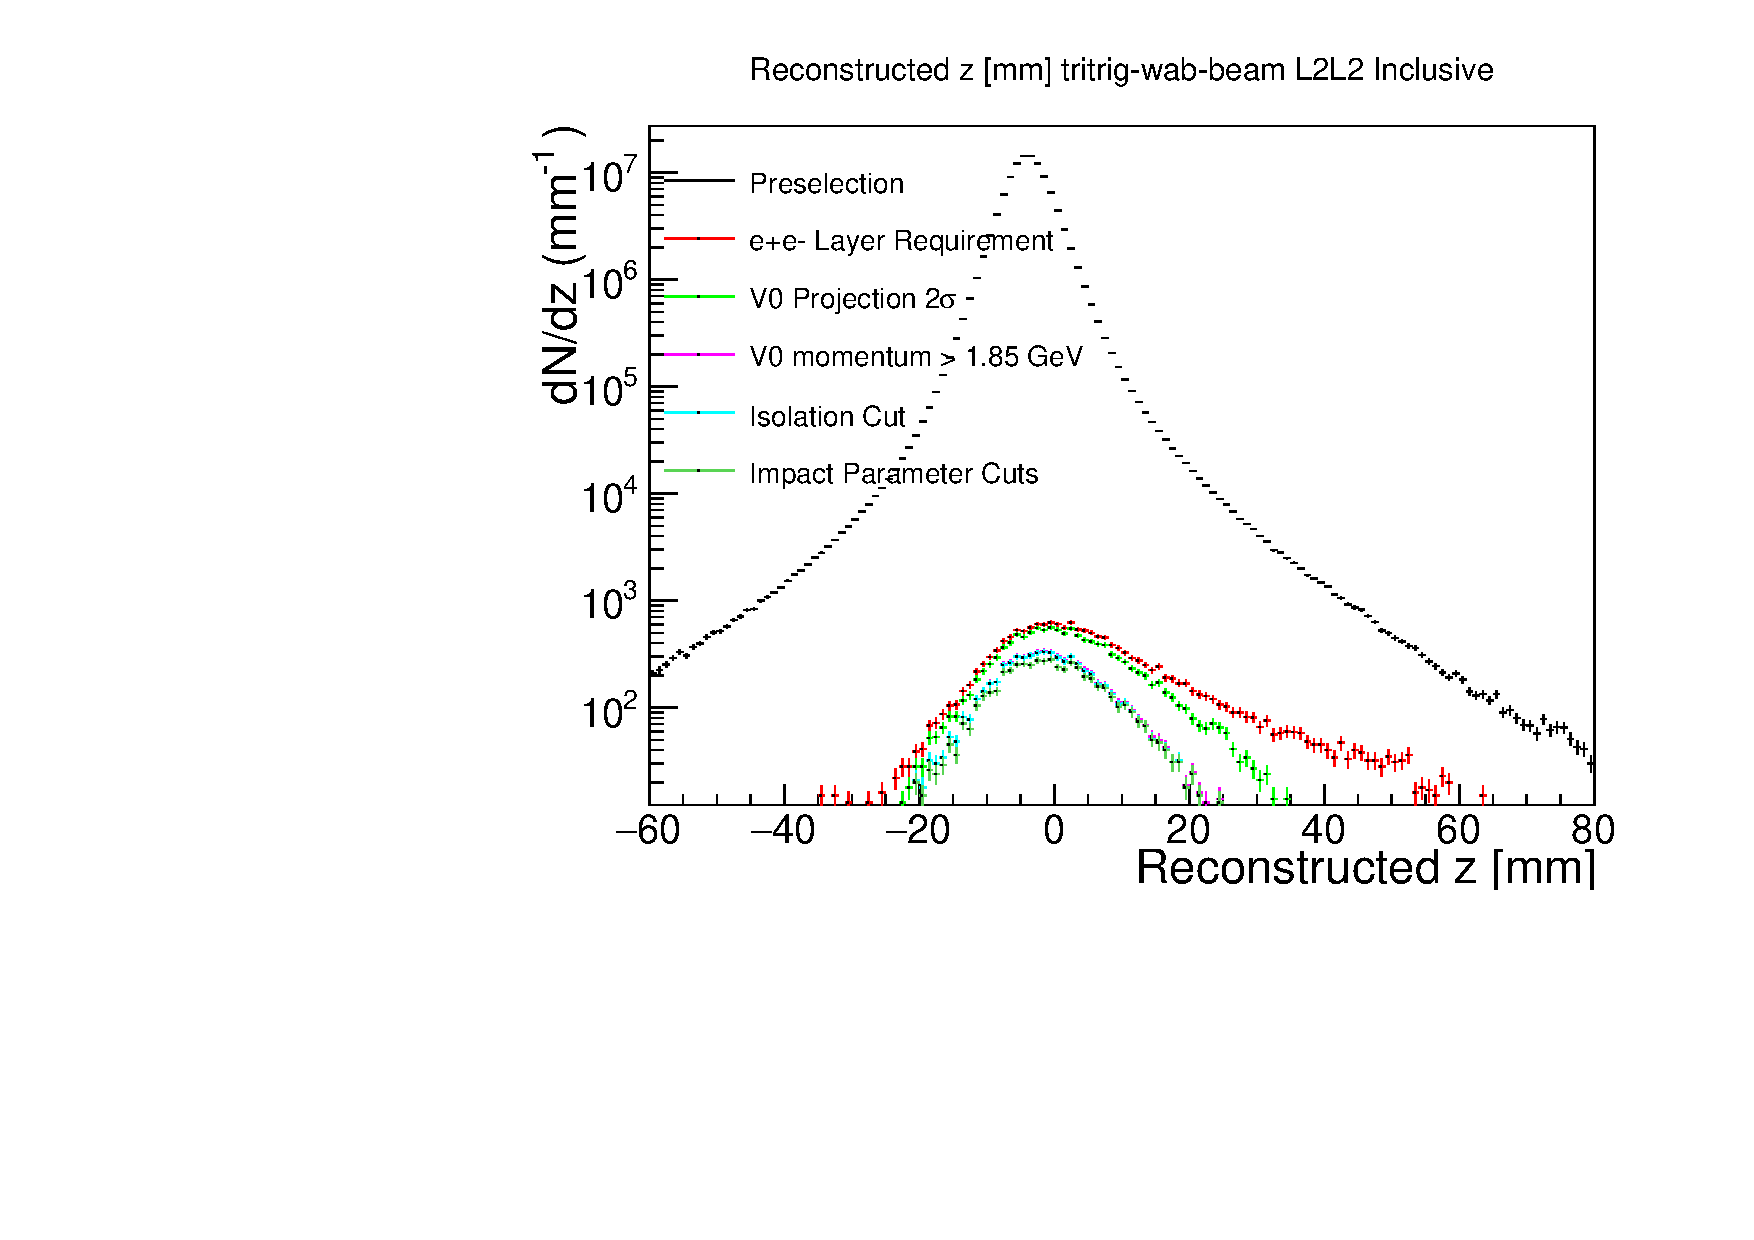
\includegraphics[width=.45\textwidth]{figs/selection/tritrig-wab-beam_L2L2_cutflow.pdf}
    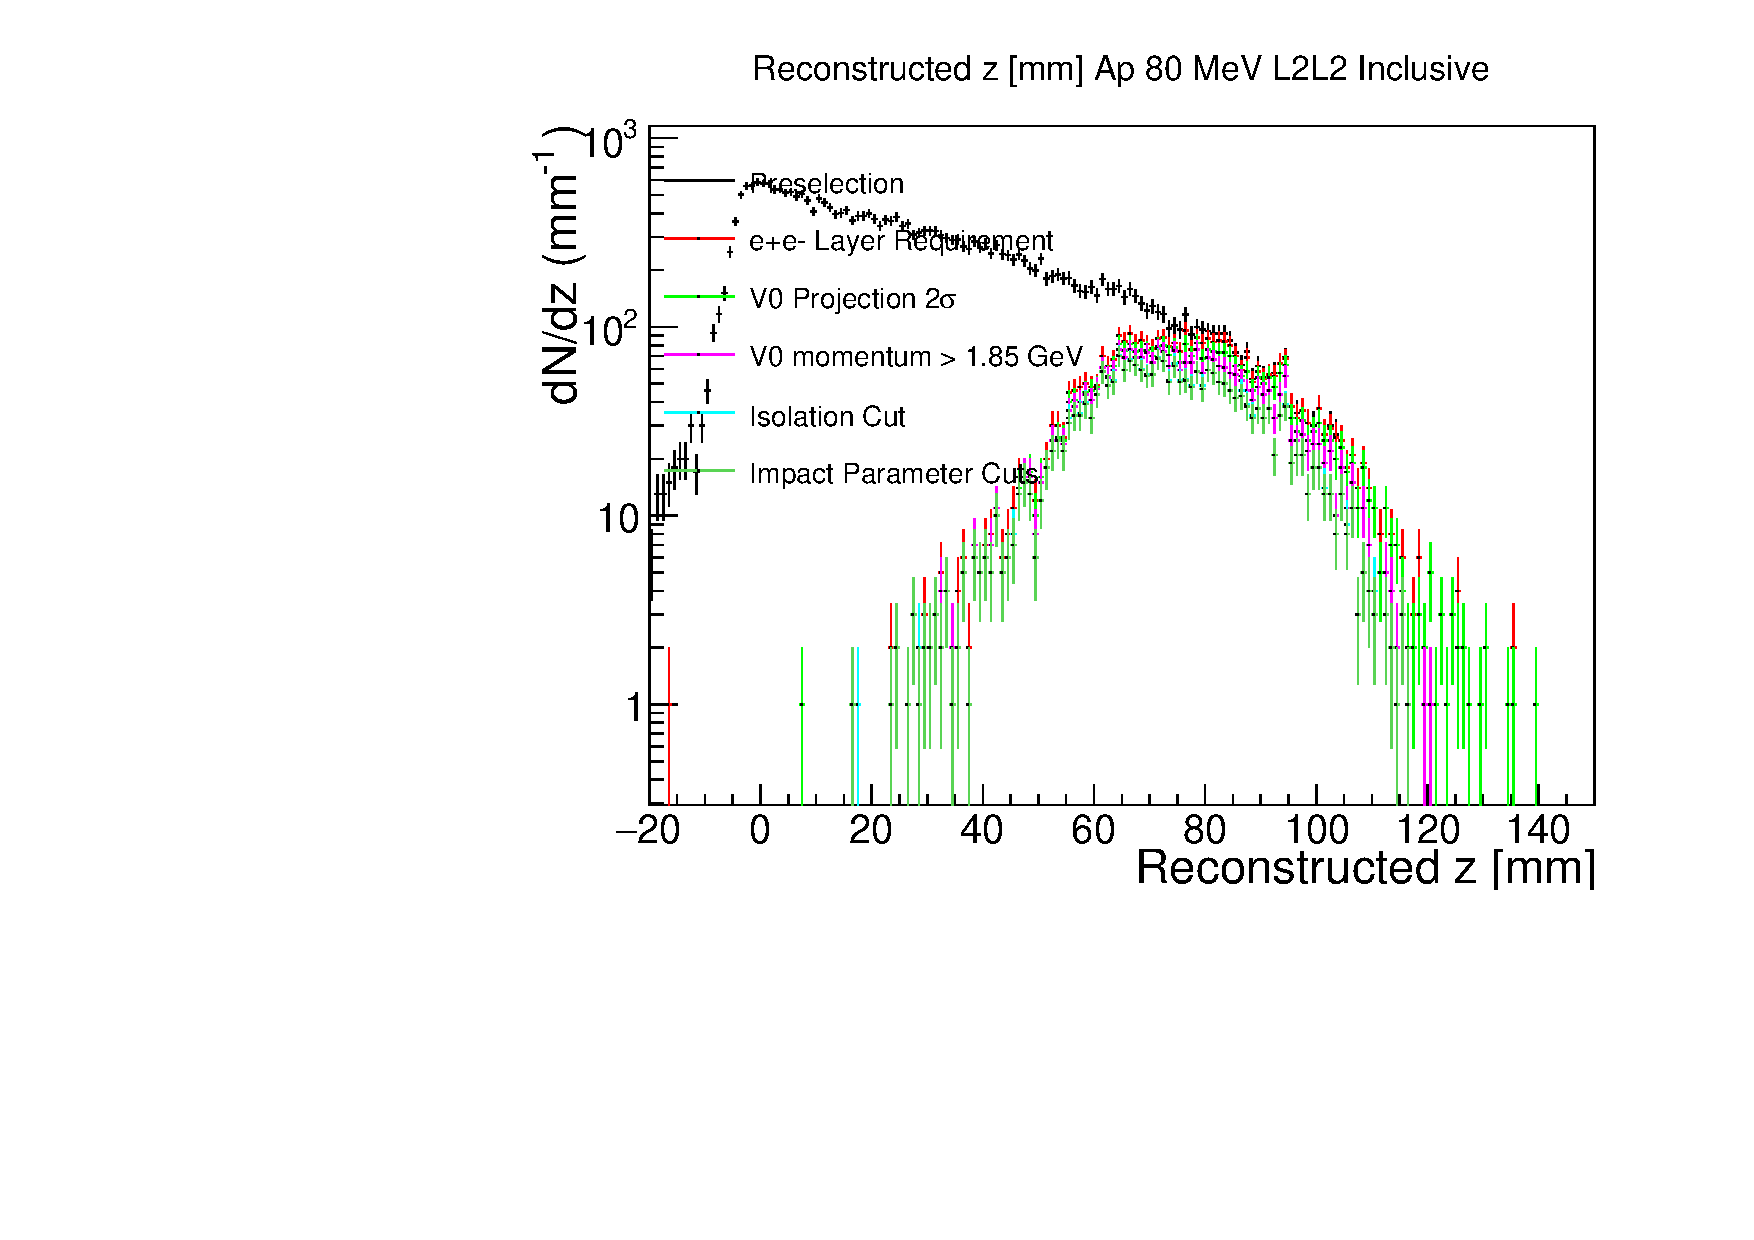
\includegraphics[width=.45\textwidth]{figs/selection/ap_80MeV_L2L2_cutflow.pdf}
    \caption{
    	Left: Cutflow for the tight event selection in the L2L2 category for 10\% of the data. Right: Cutflow for the tight selection in the L2L2 category for the full tritrig-wab-beam sample. Bottom: Cutflow for the tight event selection of a 80 MeV displaced $\aprime$. 
    }
    \label{fig:tightcutflow_L2L2}
\end{figure} 

The displaced vertex search is divided into mutually exclusive categories based on the first hit on each track of the $\epem$ pair. The so-called L1L1 and L1L2 categories were discussed in detail in Sec \ref{sec:apvertexcuts}. The remaining mutually exclusive category is the case in which both $\epem$ particles miss layer 1 of the SVT and have their first hit in the second layer. This is referred to as the L2L2 category. Much like the L1L2 category, the L2L2 category contains background events resulting from hit efficiency effects, scattering of particles in the inactive regions of the detector material, and converted WABs. The major difference between the L1L2 and L2L2 categories is that L2L2 requires one of these effects to occur for both $\epem$ pairs. 

Because of the similar nature of the backgrounds to the L1L2 category, a comparable strategy is utilized to mitigate the effects of high $z$ events in the L2L2 category. Since there must be a large opening angle for signal to be detected (as the tracker is designed at 15 mrad for prompt processes), the L2L2 category produces a much smaller signal yield across the parameter space of interest compared to the L1L1 and L1L2 categories. Because of this, the L2L2 category is excluded from the main analysis. However, as described in Sec. \ref{chap:upgrades}, the upgraded detector will have layers 1 - 3 closer to the beam plane for increased acceptance of downstream decays, and the dataset from the 2019 Physics Run includes increased luminosity that will have access to longer livetimes. This will increase the signal yield in this category, and an understanding of the backgrounds is useful for future analysis. The goal of the L2L2 analysis presented here is to perform a similar event selection and signal region definition as the L1L1 and L1L2 categories to estimate the expected signal yield (with both 10\% of the data and the full dataset) and set a limit. A basic data and MC comparison is also performed.\footnote{Data and MC agreement is not expected since hit efficiency effects and the correct WAB rates are not yet included in the MC.} This will inform us of the potential impact of the L2L2 category on the final result as well as the future work that will be necessary to obtain improved data and MC agreement and understand the high $z$ backgrounds.

\textbf{L2L2 Cutflow}

\begin{table}[!hb] 
    \centering
    \begin{tabular}{lr}
        \toprule
        \textbf{Cut Description} & \textbf{Requirement} \\
        \midrule
        Layer 1 Requirement & not $e^+$ and not $e^-$ have L1 hit \\
        Layer 2 Requirement & $e^+$ and $e^-$ have L2 hit \\
        %Tight Vertex Quality & $\chi^2_{unc} < 4$ \\
        Radiative Cut & $V_{0p} > 1.85$ GeV \\
        V0 projection to target & Fitted 2$\sigma$ cut \\
        Isolation Cut & Eq. \ref{equ:iso_final_simple_L2} \\ 
        Impact Parameters & Eq. \ref{equ:z0_cut_final} \\
        %Vertex Errors & TBD \\
        \bottomrule
    \end{tabular}
    \caption{A summary of the tight cuts for the L2L2 category.}
    \label{tab:L2L2cuts}
\end{table}

Because of the similar nature of the backgrounds from the L1L2 category, the same cuts are applied to both categories with minor changes. A rigorous approach to the actual cut values is unnecessary as this category is not a part of the standard analysis.

As with the L1L1 and L1L2 categories, the projected V0 momentum to the target is an excellent discriminator between a true displaced signal and a background that has scattered in the tracker. The pointing resolution of the momentum back to the target is degraded since the first measurement point is further from the target than layer 1 for both $\epem$ particles. Comparing the pointing resolutions from displaced $\aprime$s in the L1L1 category and the resolutions in the L2L2 category, which are roughly independent of $z$, shows a factor of 1.9 and 2.5 worse pointing resolution in the L2L2 category for the $x$ and $y$ directions, respectively. Thus, the resolutions are scaled up from the L1L1 category by a factor of 1.9 for the projection in the $x$-direction and a factor of 2.5 for the projection in the $y$-direction to match the expected resolutions in the L2L2 category. These factors cannot be derived directly from data since events in the L2L2 category are dominated by particles scattering in the layer 1 silicon, which further degrades the pointing resolutions. The fitted means from the L1L1 category are used. The cut is selected to be an elliptical cut in the $x-y$ plane at $n_{\sigma}=2$ from the mean.

Backgrounds that reconstruct at large $z$ due to mis-tracking are also present in the L2L2 category. Since neither track has a layer 1 hit, the isolation cut utilizes Eq. \ref{equ:iso_final_simple_L2}, which was derived geometrically for the case in which the first hit on track occurs in layer 2. The tuneable parameter is the number of sigma $n_{\sigma}$ on the error of the track extrapolation to the target in the vertical direction (i.e. the error on $z0$) and is set to 3.

A cut on the individual track impact parameter cut is derived in a similar way to the L1L1 and L1L2 categories using Eq. \ref{equ:z0_cut_final}. A minor difference for the L2L2 category is that there is an additional parameter for a separate $y$-intercept for top and bottom hemispheres for a total of six parameters. As with the other categories, there is a single tuneable parameter $\alpha$, the fraction of signal events that are chosen to be eliminated, which is set at 15\%.

The radiative cut is simply selected to be the same as the other categories at 1.85 GeV ($V_{0p}>1.85$ GeV). Finally, tracks with shared hits are eliminated, and events which still contain more than one V0 candidate after all cuts are eliminated. A summary of the cuts is shown in Table \ref{tab:L2L2cuts} and the cutflow is shown in Fig. \ref{fig:tightcutflow_L2L2}. The final selection for both data and MC is shown in Fig. \ref{fig:final_zcut_L2L2}.%\ref{fig:singleV0_2D_L1L2}.

%\begin{figure}[!ht] 
%    \centering
%    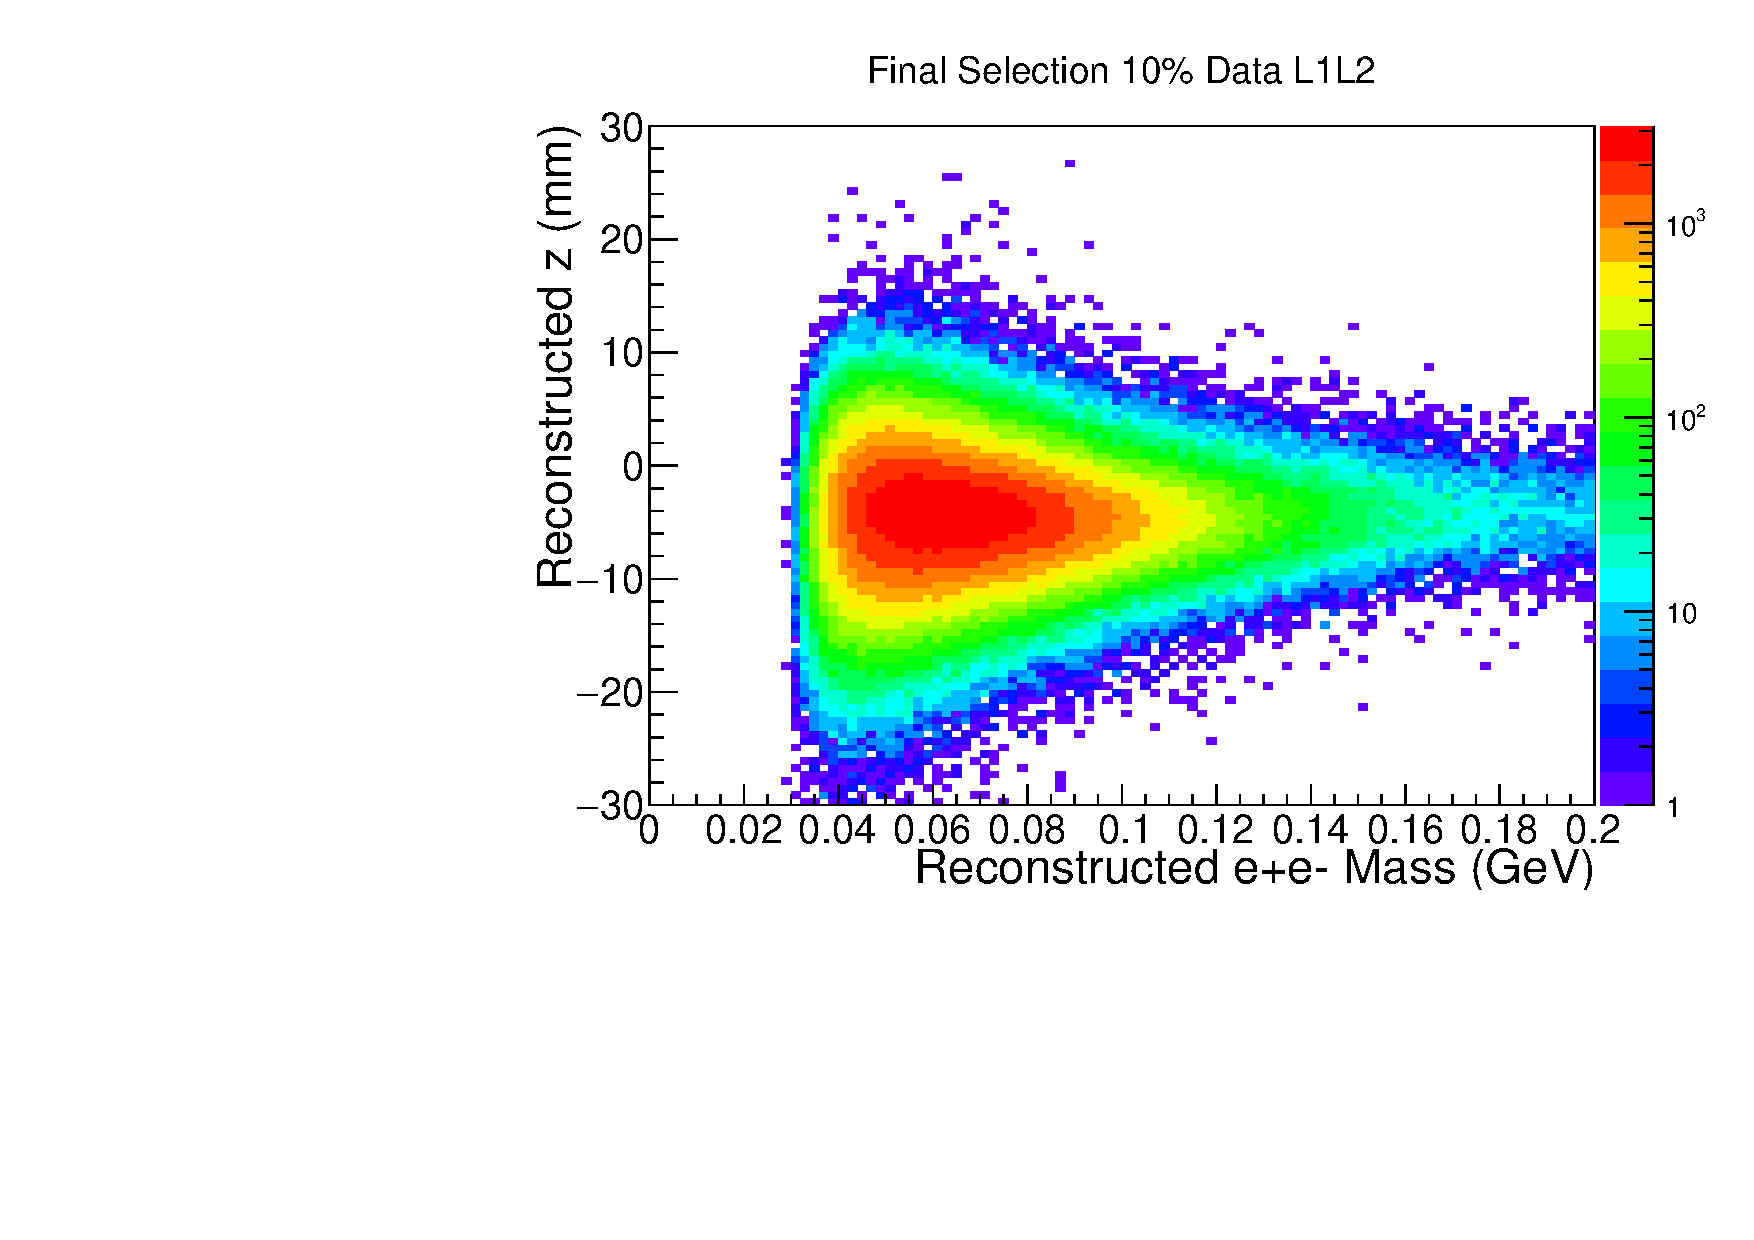
\includegraphics[width=.45\textwidth]{figs/selection/data_L1L2_final_vz_mass.pdf}
%    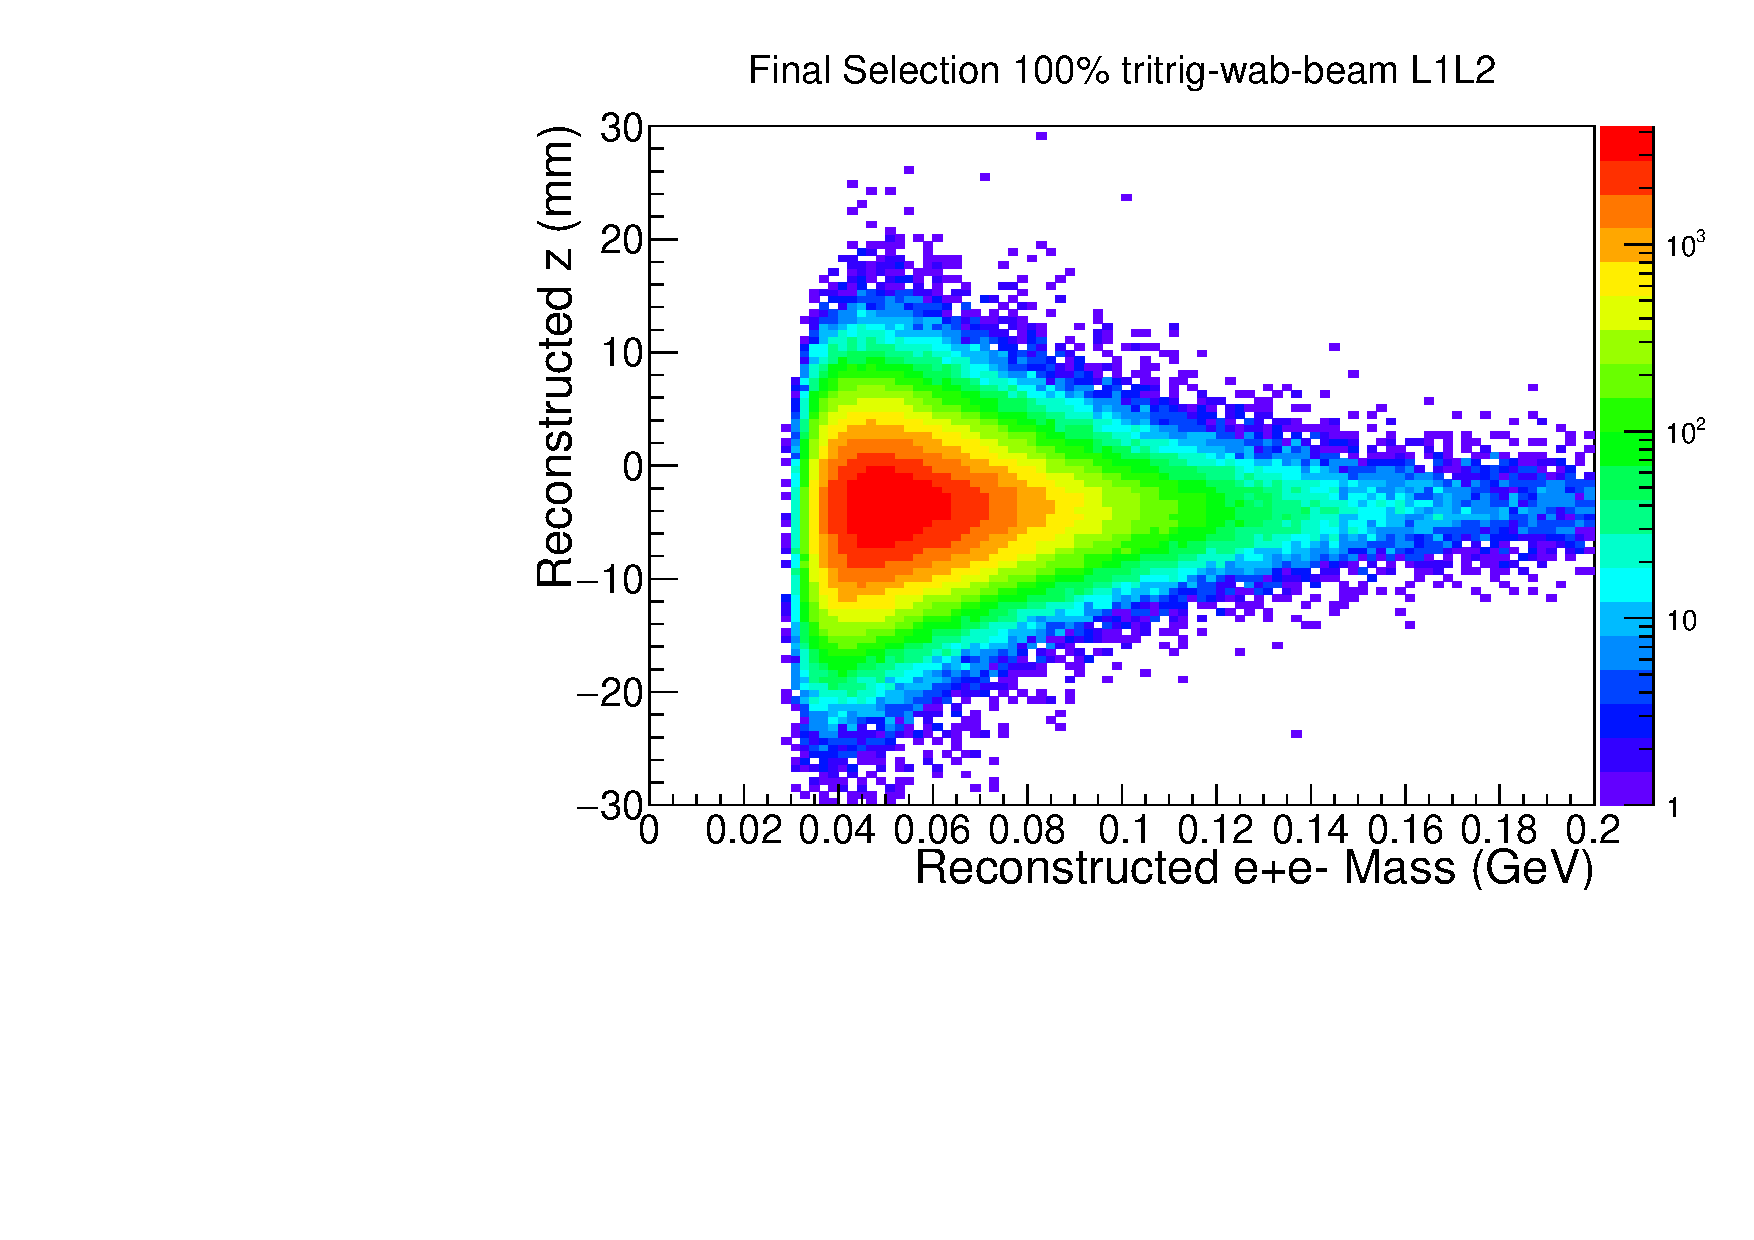
\includegraphics[width=.45\textwidth]{figs/selection/mc_L1L2_final_vz_mass.pdf}
%    \caption{
%    	Left: Reconstructed $z$ vs. reconstructed $\epem$ mass for the final selection in 10\% of the data for the L2L2 category. Right: Reconstructed $z$ vs. reconstructed $\epem$ mass for the final selection for the full tritrig-wab-beam MC sample for the L2L2 category.
%    	\textcolor{red}{Update plots with L2L2.}
%    }
%    \label{fig:singleV0_2D_L2L2}
%\end{figure}  

\begin{figure}[t]
    \centering
    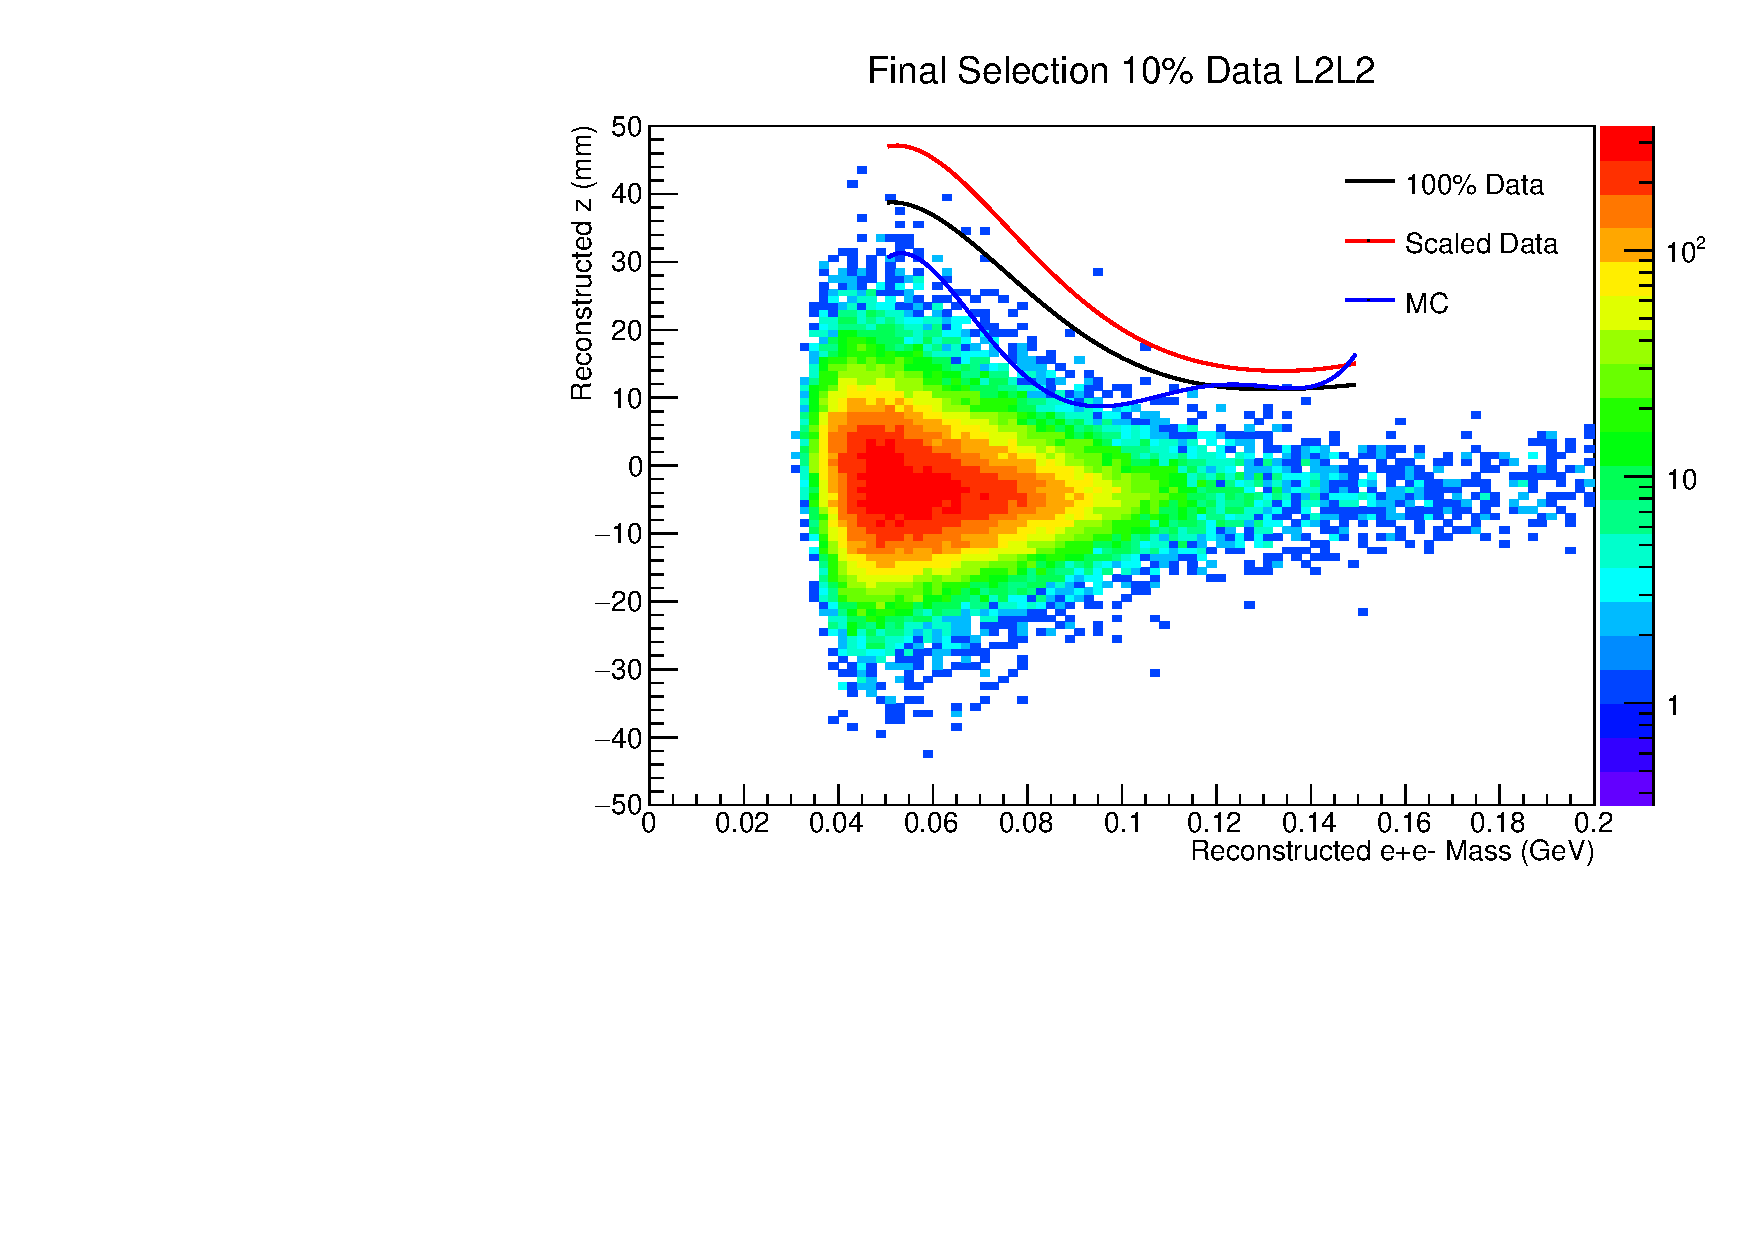
\includegraphics[width=.85\textwidth]{figs/Results/10per_L2L2_final_zcut.pdf}
    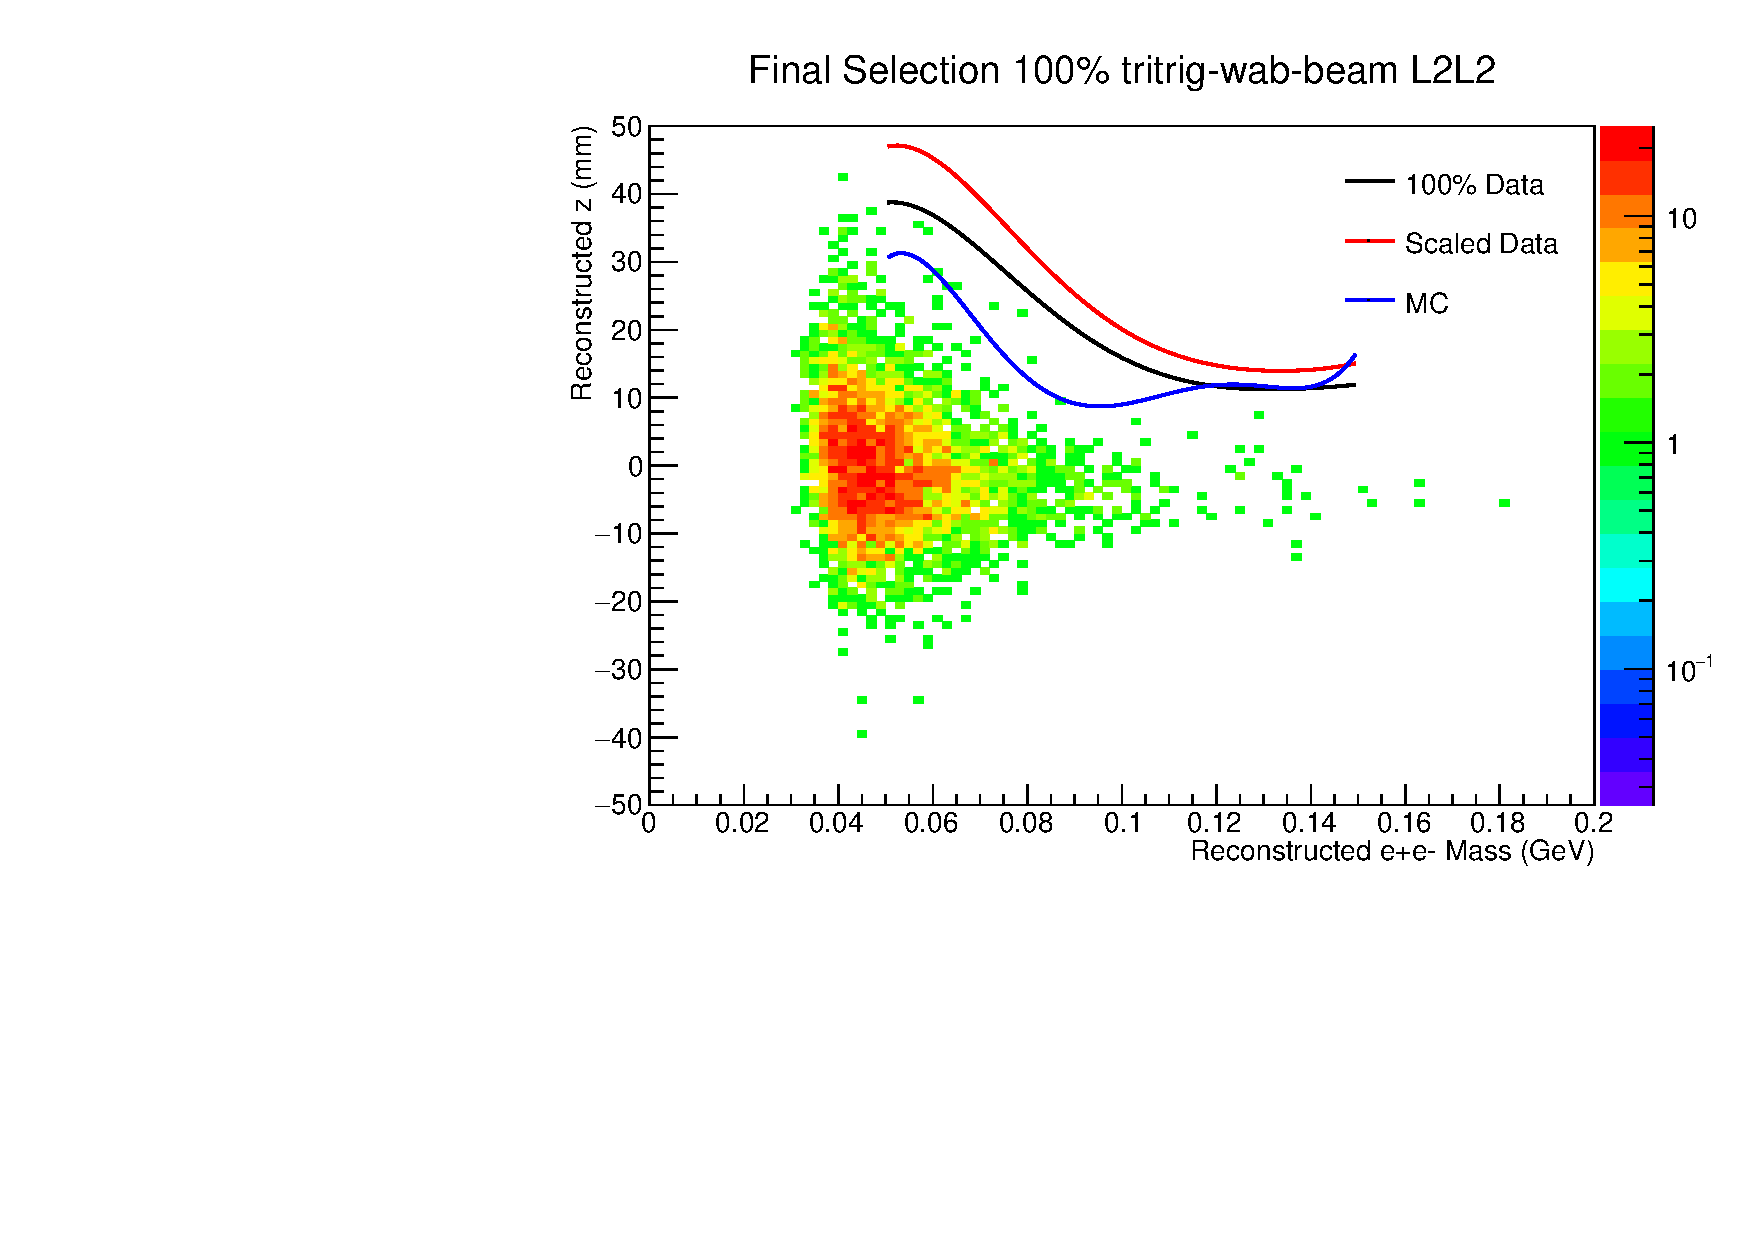
\includegraphics[width=.85\textwidth]{figs/Results/tritrig-wab-beam_L2L2_final_zcut.pdf}
    \caption{The final event selection with overlaid $z_{cut}$ from 10\% data, the full tritrig-wab-beam sample, and projected to the full dataset for Top: 10\% data for the L2L2 category and Bottom: full tritrig-wab-beam sample for the L2L2 category. The 10\% data sample contains $\sim10^6$ events while the full tritrig-wab-beam sample contains about $\sim5 \times 10^{3}$ events.}
    \label{fig:final_zcut_L2L2}
\end{figure}

\clearpage

\textbf{L2L2 Final Results}

The final results for the L2L2 category, which includes computing the expected yield and setting a limit, is done using a similar method to the other categories. First, the mass resolution is parameterized with the same track momentum smearing method described in Sec \ref{sec:massresolution} (the smearing constant for 5-hit tracks is used). The mass resolution parametrization is shown in Fig. \ref{fig:mres_L2L2} and is used to determine the size of the search windows ($1.9\sigma_m$).

\begin{figure}[t]
    \centering
    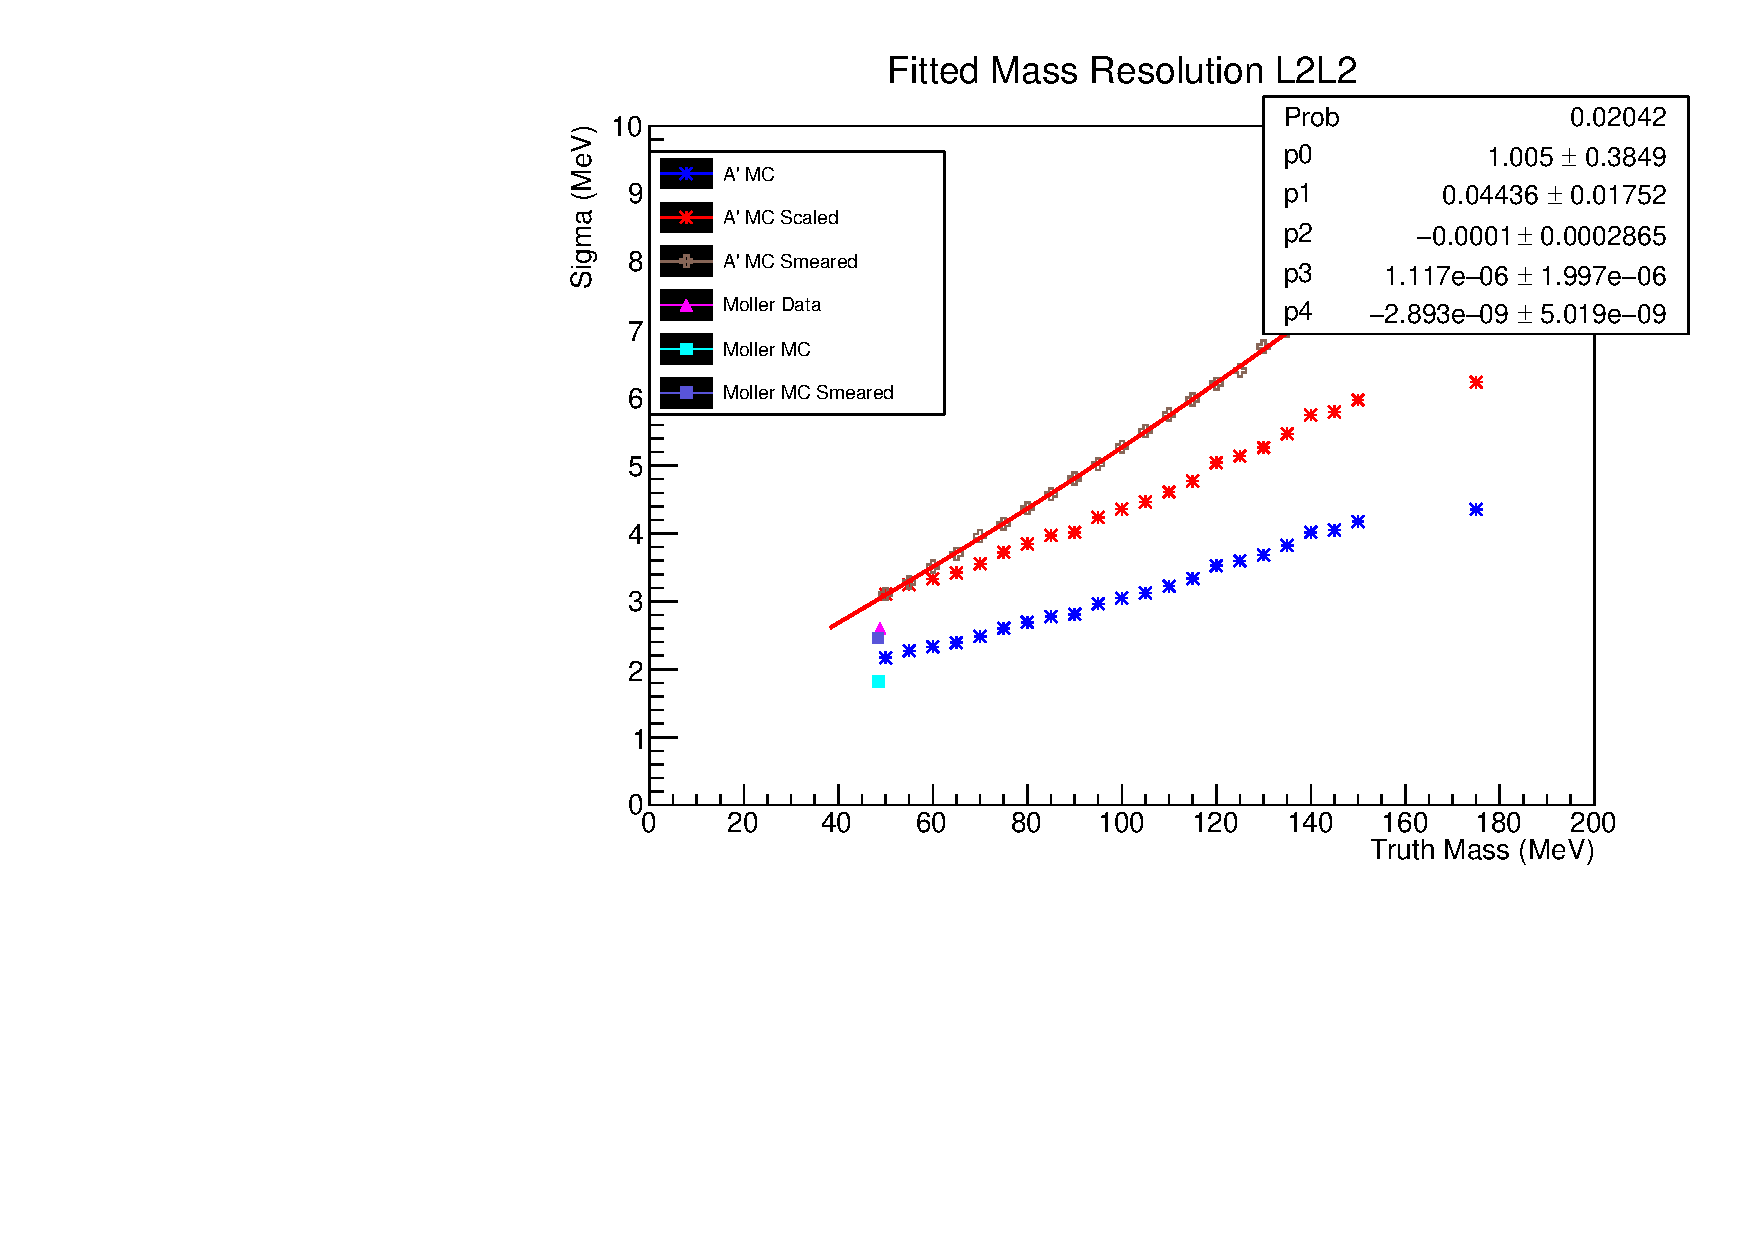
\includegraphics[width=.45\textwidth]{figs/Results/massRes_L2L2.pdf}
    \caption{The parametrization of the mass resolution for the L2L2 category as a function of $\aprime$ mass. The method uses the smearing track momentum method to re-scale the mass resolution described in Sec \ref{sec:massresolution}, but exclusively using 5-hit tracks.}
    \label{fig:mres_L2L2}
\end{figure}

The efficiency as a function of reconstructed $z$ is derived from the method utilizing the track slope-dependent hit killing algorithm described in Sec. \ref{sec:aprimerate}. Since the hit killing algorithm only operates on layer 1, the L2L2 category can only gain events from both the L1L1 and L1L2 categories.

The signal region at $z(m)>z_{cut}(m)$ is defined by using the background fit in Eq. \ref{eqn:tail_fit} and solving for the corresponding $z_{cut}$ at 0.5 expected background events. The $z_{cut}$ as a function of mass overlaid on the final events selection is shown in Fig. \ref{fig:final_zcut_L2L2} for both data and MC. In general, this fit has a much longer tail than the background fits in the L1L1 and L1L2 categories, and in the future, this background fit for the L2L2 category will be more thoroughly explored.

The expected $\aprime$ signal yield is computed using Eq. \ref{eqn:signal_yield} and is shown for 10\% of the data and the projected full dataset in Fig. \ref{fig:sigyield_L2L2}. For 10\% of the data, the peak expected signal yield is 0.01 events at a mass of 74.7 MeV and $\epsilon^2=1.05 \times 10^{-9}$. Scaled up to the full dataset, the projected peak value is 0.05 $\aprime$ events at 72.9 MeV and the same $\epsilon^2$. Finally, a limit is set using the Optimum Interval Method and the results on the full dataset for L2L2 is shown in Fig. \ref{fig:OIM_L2L2}. For 10\% of the data, the optimum exclusion is at a value of 420.7 times the canonical $\aprime$ cross-section at a mass of 72.9 MeV and $\epsilon^2=1.05 \times 10^{-9}$. This result contributes $\sim$10\% to the overall signal yield when added to the results of the L1L1 and L1L2 categories. And because of this relatively small contribution in conjunction with several outstanding issues to solve, the L2L2 category is not included as part of the standard analysis.

\begin{figure}[t]
    \centering
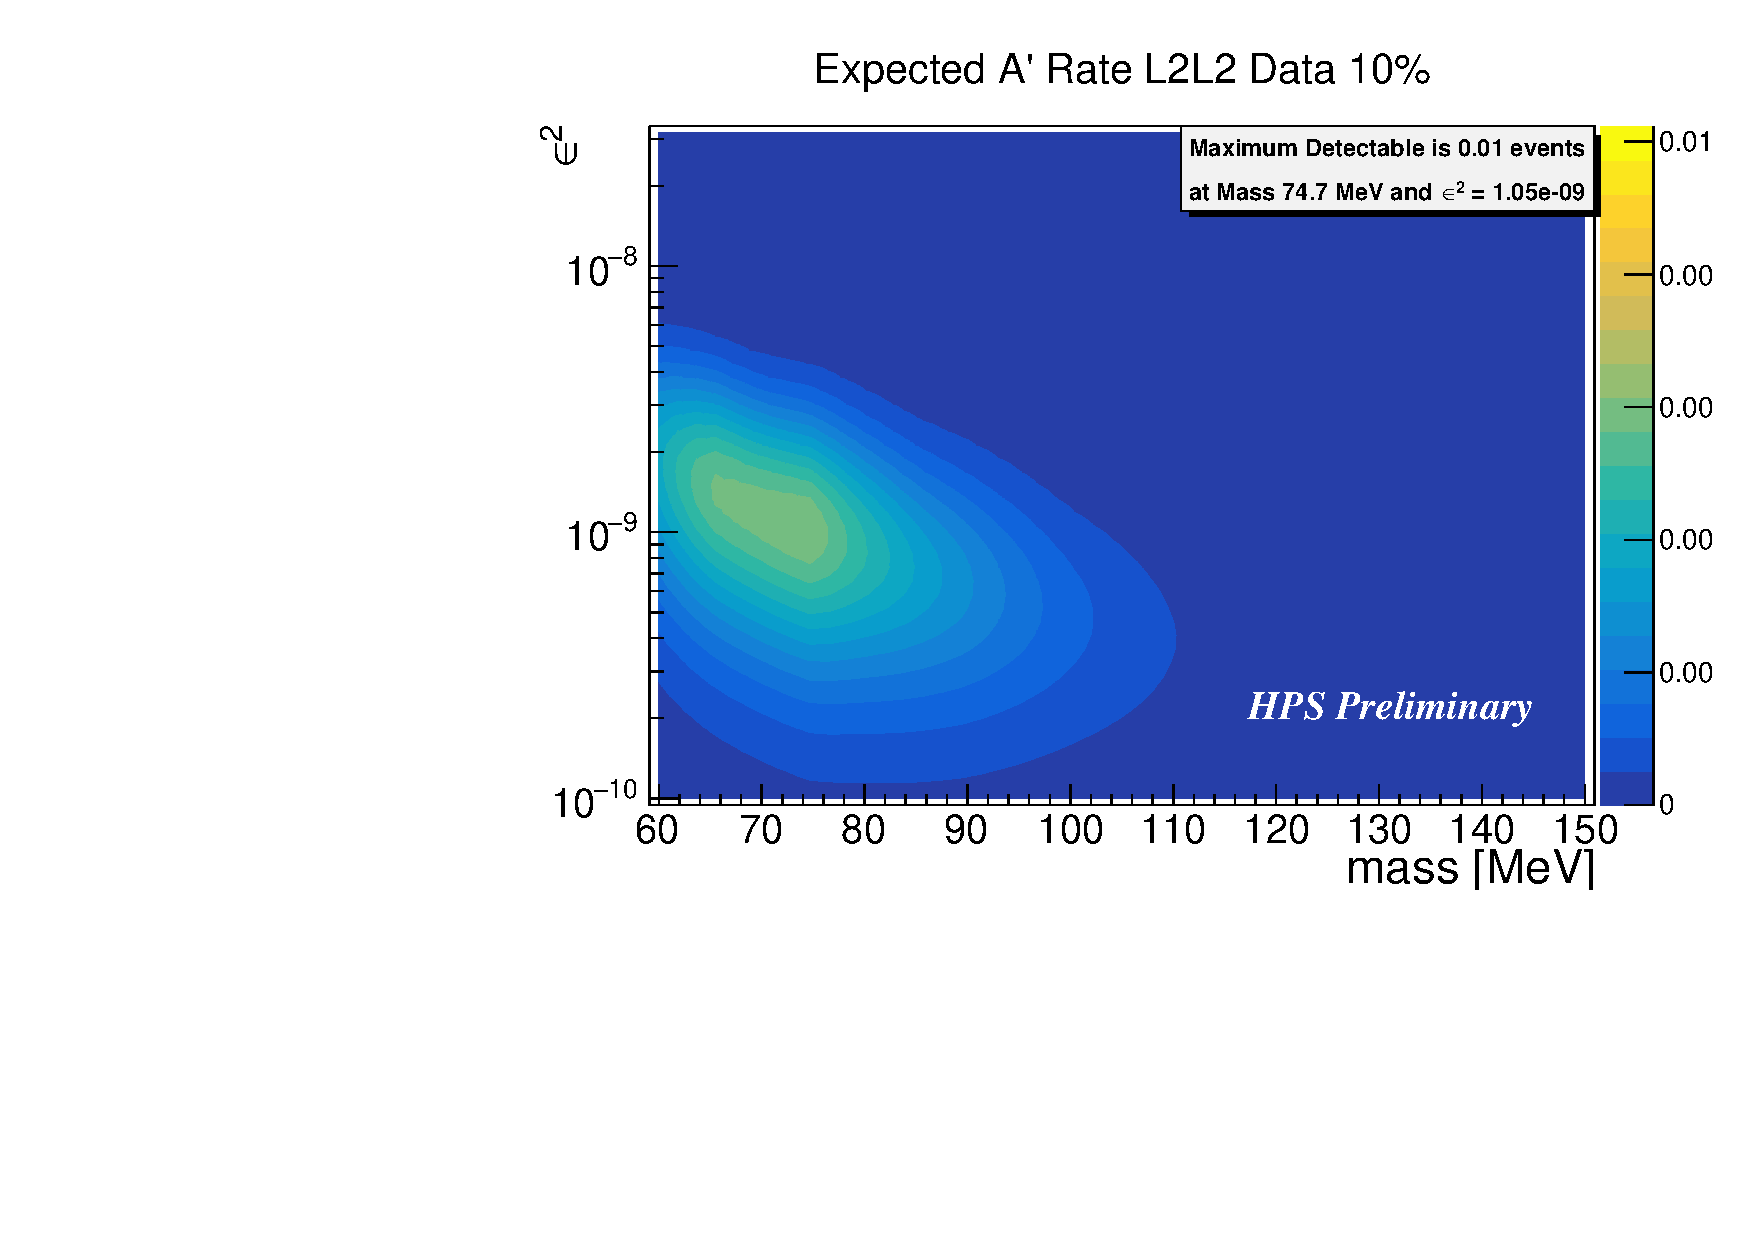
\includegraphics[width=.85\textwidth]{figs/Results/ap_rate_L2L2.pdf}
    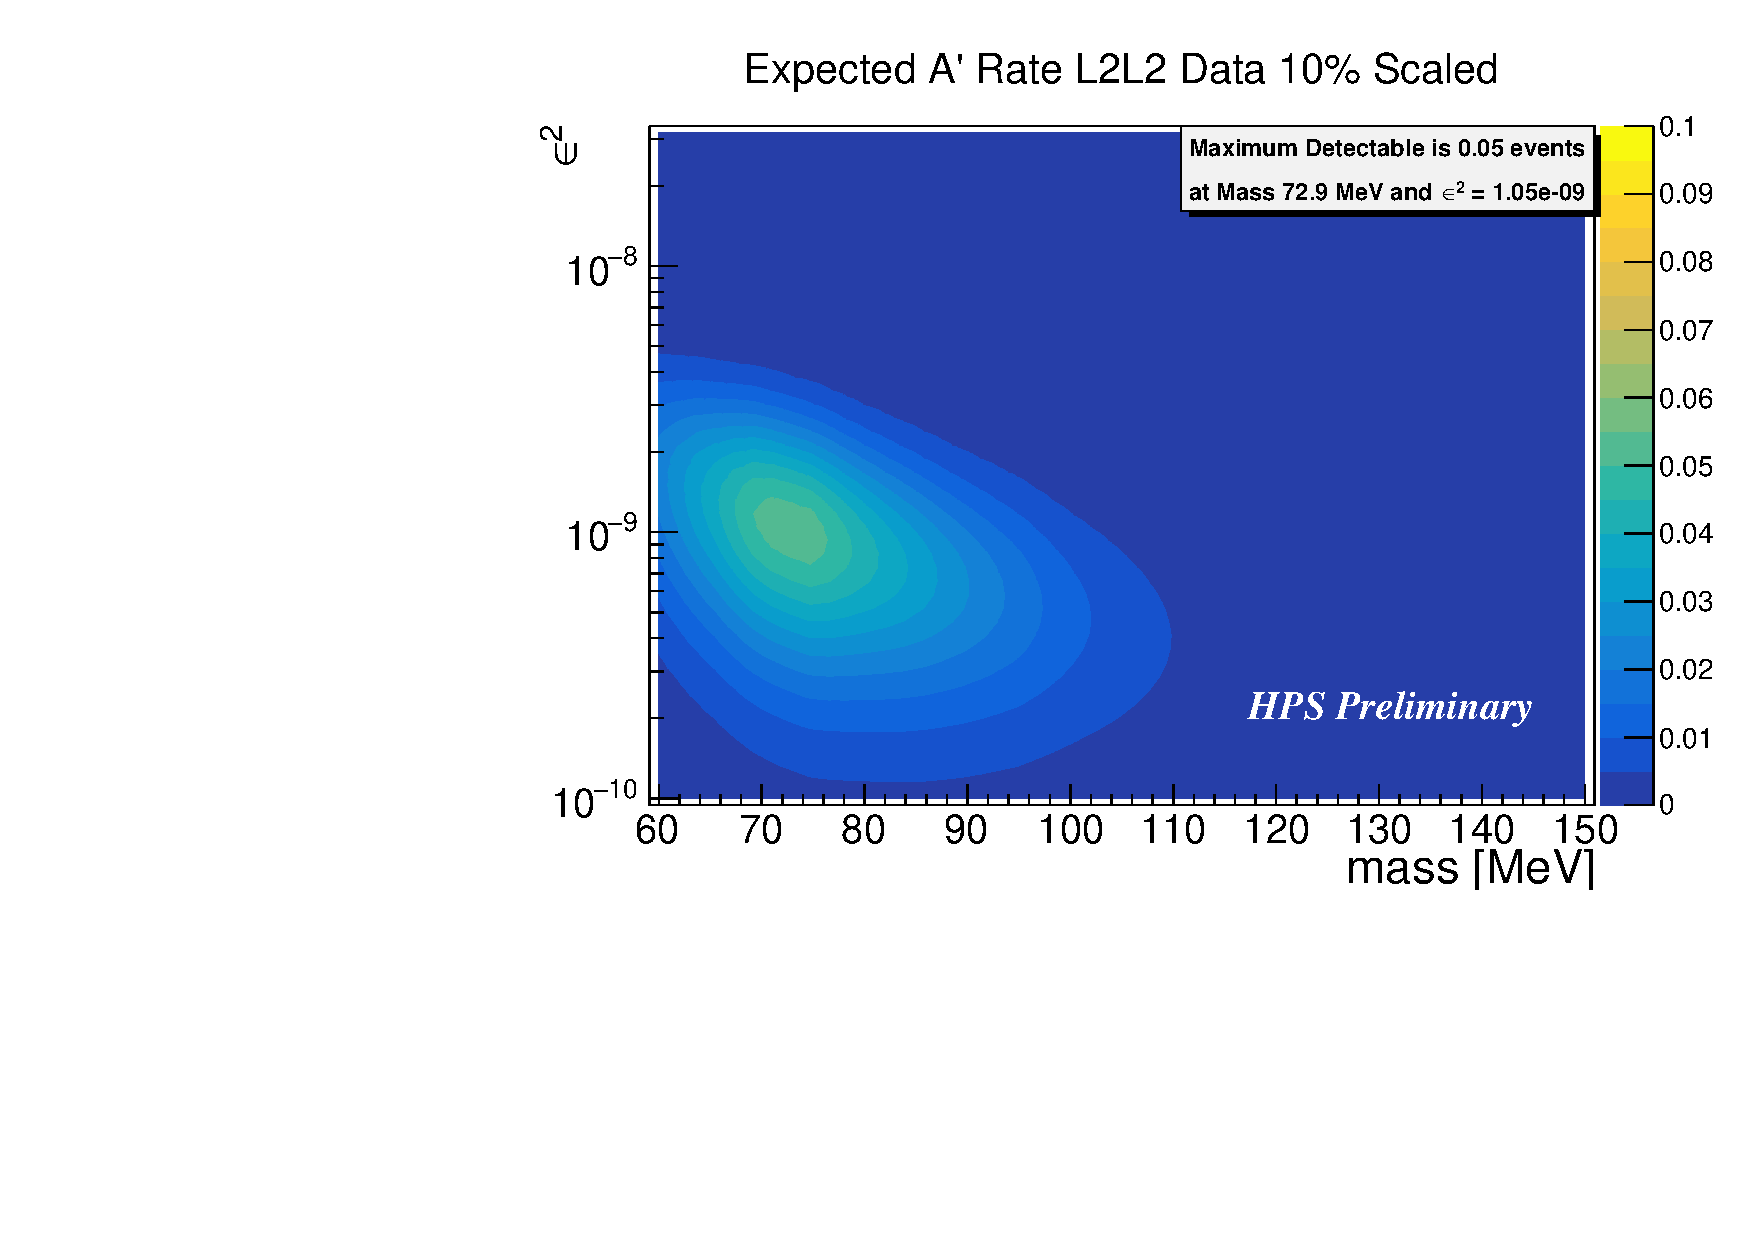
\includegraphics[width=.85\textwidth]{figs/Results/ap_rate_L2L2_scaled.pdf}
    \caption{Top: The expected number of $\aprime$ events past $z_{cut}$ including all efficiencies for the L2L2 category for 10\% of the data. Bottom: The expected number of $\aprime$ events past $z_{cut}$ including all efficiencies for the L2L2 category projected for the full dataset. }
    \label{fig:sigyield_L2L2}
\end{figure}

\begin{figure}[t]
    \centering
    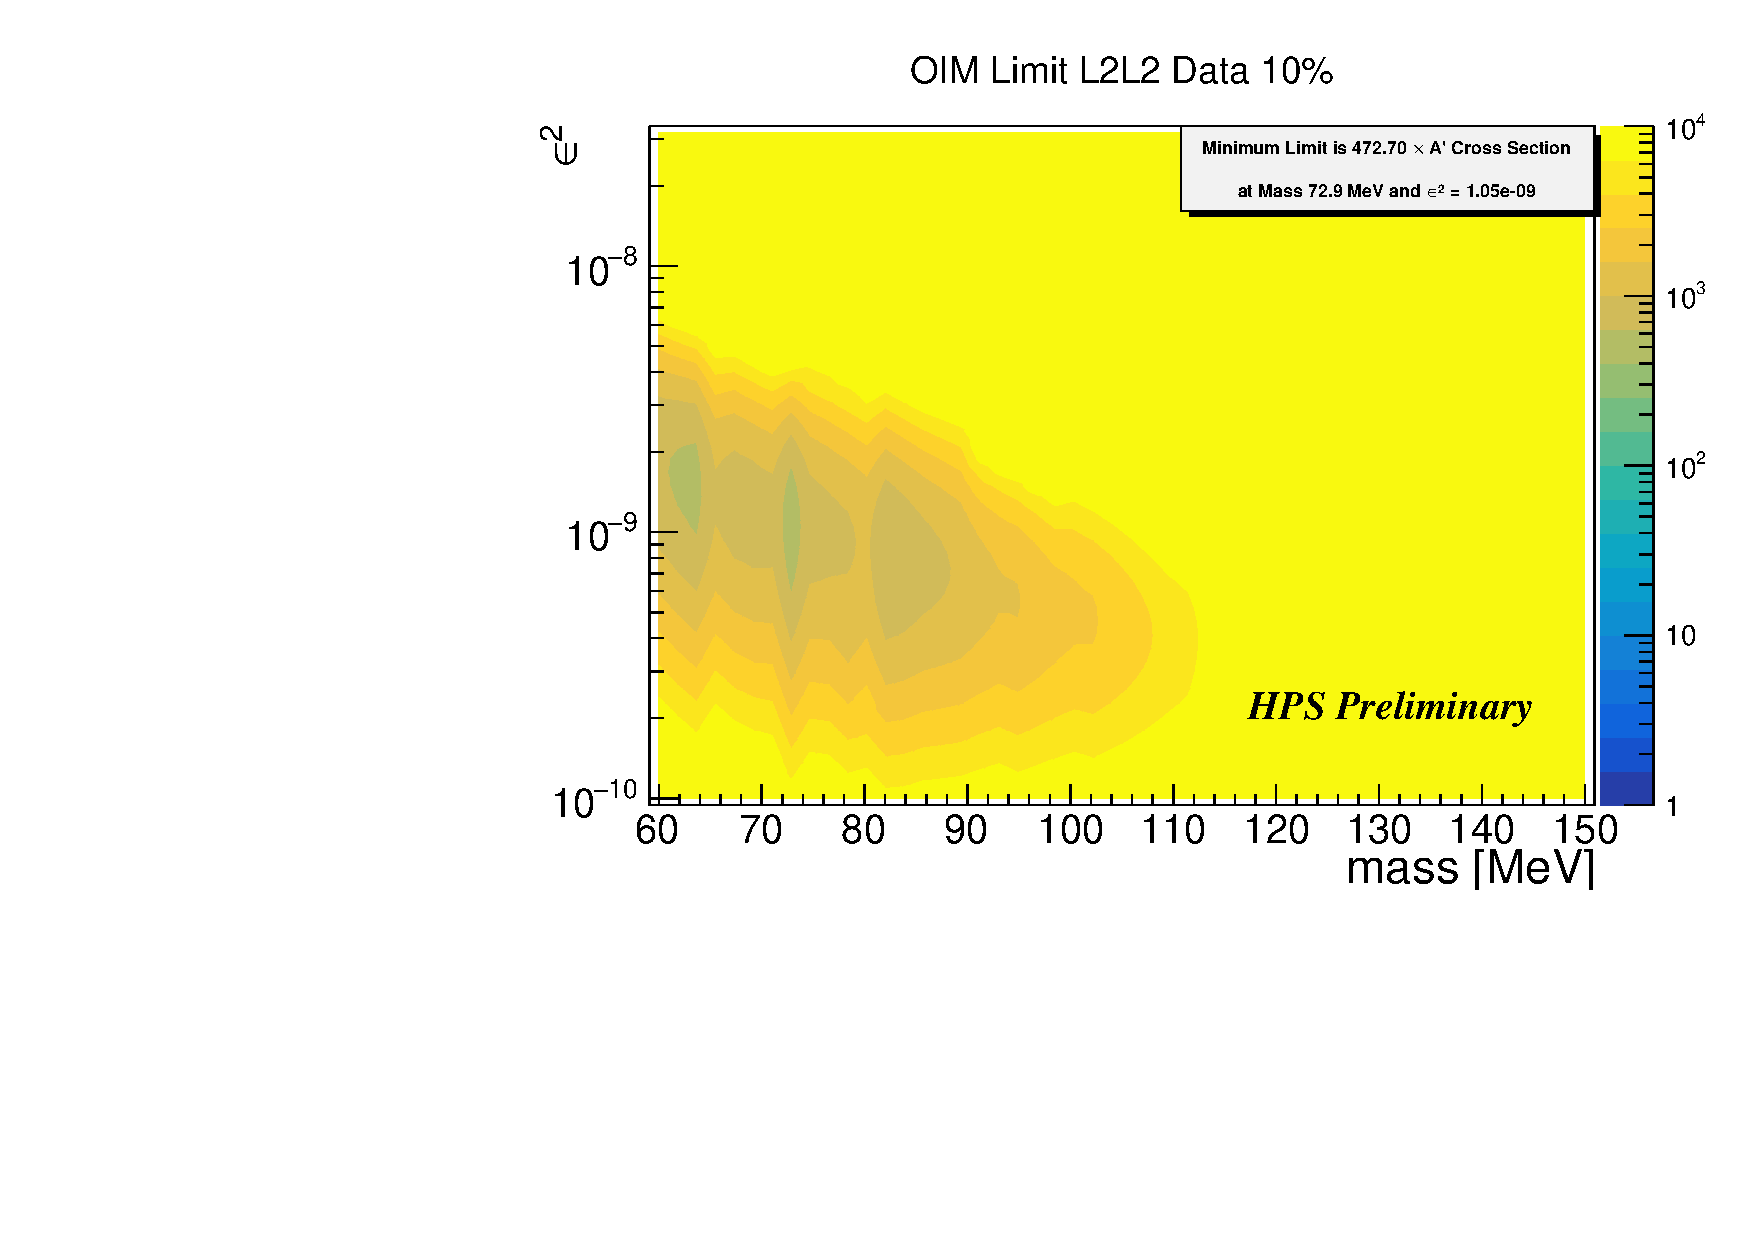
\includegraphics[width=.85\textwidth]{figs/Results/oim_L2L2.pdf}
    \caption{The limit from Optimum Interval Method for the L2L2 category. }
    \label{fig:OIM_L2L2}
\end{figure}

\clearpage

\textbf{Discussion of High $z$ Events in L2L2}

High $z$ events are present in the L2L2 subset of the data. Unfortunately, similar to the L1L2 category, there is poor agreement between data and MC for both the overall rate and the pattern of high $z$ events. This is of course a result of an ad hoc method of incorporating hit efficiency effects and the incorrect fraction of WABs in the tritrig-wab-beam sample as discussed in Sec. \ref{sec:apL1L2}. A summary of the variables of interest for the high $z$ events in the L2L2 category are shown in Table \ref{tab:highZ_L2L2_unblind} for the full dataset and in Table \ref{tab:highZ_L2L2_tritrig-wab-beam} for the full MC. Similar to the L1L2 categories, the L2L2 for data contains many high $z$ events that have a large vertex $\chi^2$ or reconstruct far from the beam plane in the $y$-direction, and thus are not signal-like. MC shows some large scattering away from the beam plane in layer 1, although since neither of these particles have a layer 1 hit, it is necessary to check the scattering in layer 2.


\begin{table}[t]
\centering
\tabcolsep=0.09cm
%\begin{tabular}{lrlrlrlrlrl}
\begin{tabular}{lllllllllll}

\hline

$\Delta z_{cut}$ & VZ (mm) & Mass (MeV) & Run & Event & $\chi^2_{unc}$ & V0 Proj Y ($n_{\sigma}$) & VY ($n_{\sigma}$) & $\Delta \ e^- \ z0$ (mm) & $\Delta \ e^+ \ z0$ (mm) \\
2.83 & 34.47 & 70.24 & 7644 & 230616 & 5.76 & 1.55 & 6.34 & 0.70 & 3.12 \\ 
24.15 & 51.22 & 77.75 & 7780 & 73604033 & 0.96 & 0.71 & 4.66 & 1.95 & 3.26 \\
19.99 & 52.96 & 67.95 & 7804 & 108519861 & 9.45 & 1.12 & 0.90 & 2.13 & 2.40 \\ 
10.99 & 28.89 & 94.88 & 8044 & 61348427 & 0.11 & 1.49 & 1.18 & 1.81 & 1.33 \\ 3.44 & 39.25 & 62.53 & 8057 & 40390234 & 7.13 & 0.07 & 6.05 & 0.38 & 1.84 \\ 
2.92 & 17.27 & 104.92 & 8099 & 4969709 & 4.36 & 1.38 & 3.11 & 0.49 & 1.50 \\ 
\hline

\hline
\end{tabular}
\caption{A table of relevant variables for events past $z_{cut}$ for 10\% of the data in the L2L2 category. Events in which $V_z>80$ mm have been removed since it is expected that these originated from tridents produced in the first silicon layer as discussed in the text.}
\label{tab:highZ_L2L2_unblind}
\end{table}


\begin{table}[t]
\centering
\tabcolsep=0.09cm
%\begin{tabular}{lrlrlrlrlrl}
\begin{tabular}{lllllllllll}

\hline

$\Delta z_{cut}$ & VZ (mm) & Mass (MeV) & $\theta_{1}$ (mrad) & $\theta_{2}$ (mrad) & $\chi^2_{unc}$ & V0 Proj Y ($n_{\sigma}$) & VY ($n_{\sigma}$) & $\Delta \ e^- \ z0$ (mm) & $\Delta \ e^+ \ z0$ (mm) \\
8.20 & 22.23 & 78.25 & 0.59 & 2.52 & 6.65 & 1.26 & 2.27 & 0.65 & 1.35 \\ 
5.06 & 23.00 & 72.97 & 1.94 & 10.57 & 7.31 & 1.50 & 2.40 & 0.97 & 0.84 \\ 
2.81 & 15.18 & 81.02 & 2.12 & 1.56 & 0.20 & 0.07 & 1.19 & 0.75 & 0.32 \\ 
1.47 & 26.74 & 64.54 & 2.55 & 7.75 & 0.64 & 0.33 & 3.52 & 1.03 & 0.63 \\

\hline

\hline
\end{tabular}
\caption{A table of relevant variables for events past $z_{cut}$ for the full tritrig-wab-beam sample in the L2L2 category. Events that have been added to the L2L2 category from hit inefficiencies in the L1L1 and L1L2 categories are not included in this table.}
\label{tab:highZ_L2L2_tritrig-wab-beam}
\end{table}

A major source of high $z$ backgrounds is trident production in the silicon from a beam electron that is elastically scattered in the target. This is evident in the 3D positions of the vertex which are consistent with the physical location of the sensors. In particular, one can see the offset of the four layer one sensors - top axial/stereo and bottom stereo/axial located at a $z$-position of about 87 mm, 97 mm, 103 mm, and 113 mm, respectively - along with a reconstructed $y$-position which is significantly far from the beam plane. This can be seen clearly in Fig. \ref{fig:yz_L2L2}. In principle, a simple geometrical cut can eliminate these events, though with some loss to signal efficiency. Trident production in the silicon is not currently simulated. One such event is seen in 10\% of the data in the L1L2 category which is less common since the L1L2 category requires a layer 1 hit.

Of course the last possible explanation of high $z$ events is a displaced signal. It is unlikely based on the small number of expected $\aprime$ events. Any potential signal must be tested against the expected exponential distribution and against the L1L1 and L1L2 categories in which more events are typically expected.

\begin{figure}[t]
    \centering
    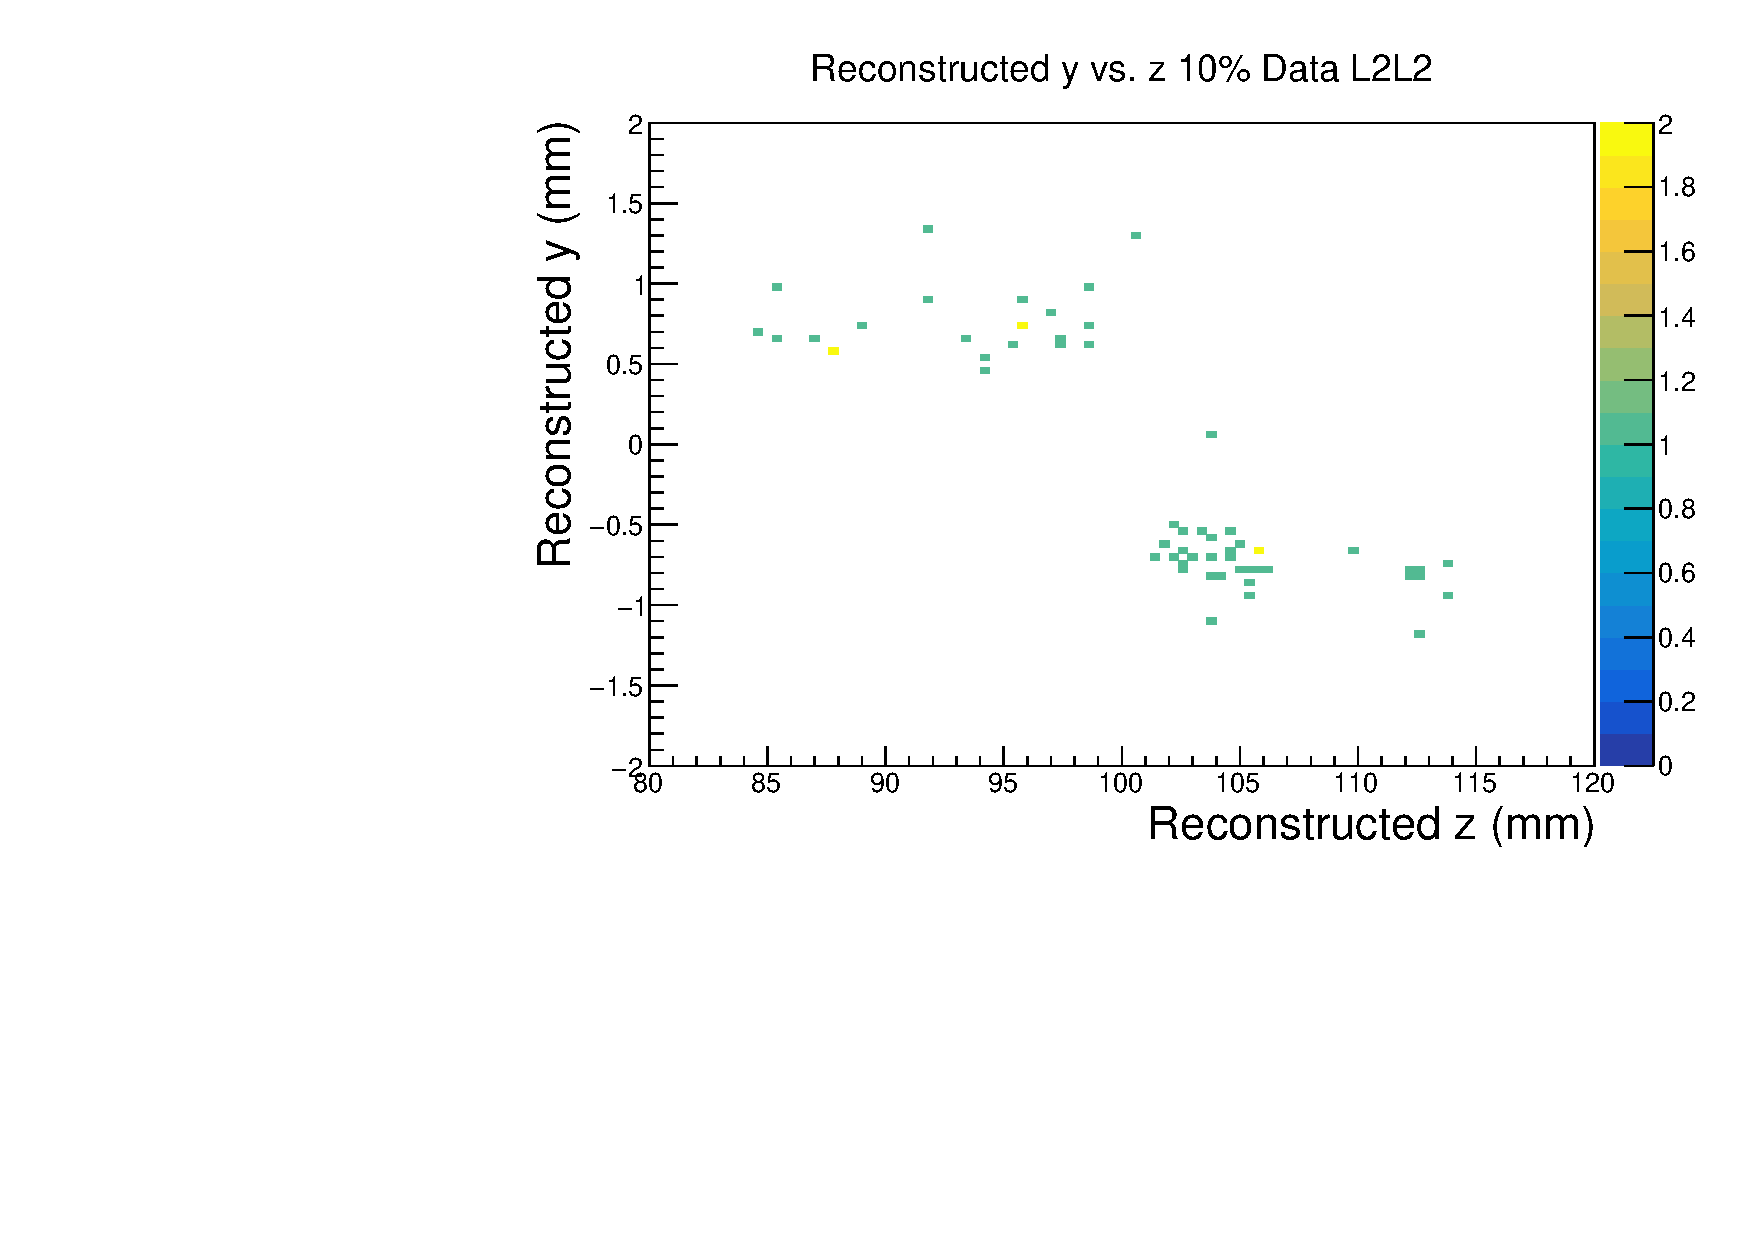
\includegraphics[width=.85\textwidth]{figs/Results/y_z_L2L2.pdf}
    \caption{The reconstructed $y$ vs. the reconstructed $z$ for events that reconstruct significantly downstream of the target in the L2L2 category in the 10\% sample in data. These events are most likely a result of trident production in the layer 1 silicon from a beam particle that elastically-scattered in the target. The is most evident in the top/bottom $z$ offset, which is present in the SVT design. Trident production in the silicon is not currently simulated.}
    \label{fig:yz_L2L2}
\end{figure}